\section{Oszillator x2 \label{Osci}}
\label{sec:org425d810}
Dieses Modul ist ein simples signalerzeugendes Modul, welches zwei voneinander unabhängige Rechteckswellen im hörbaren Bereich generiert.

\begin{figure}[htbp]
\centering
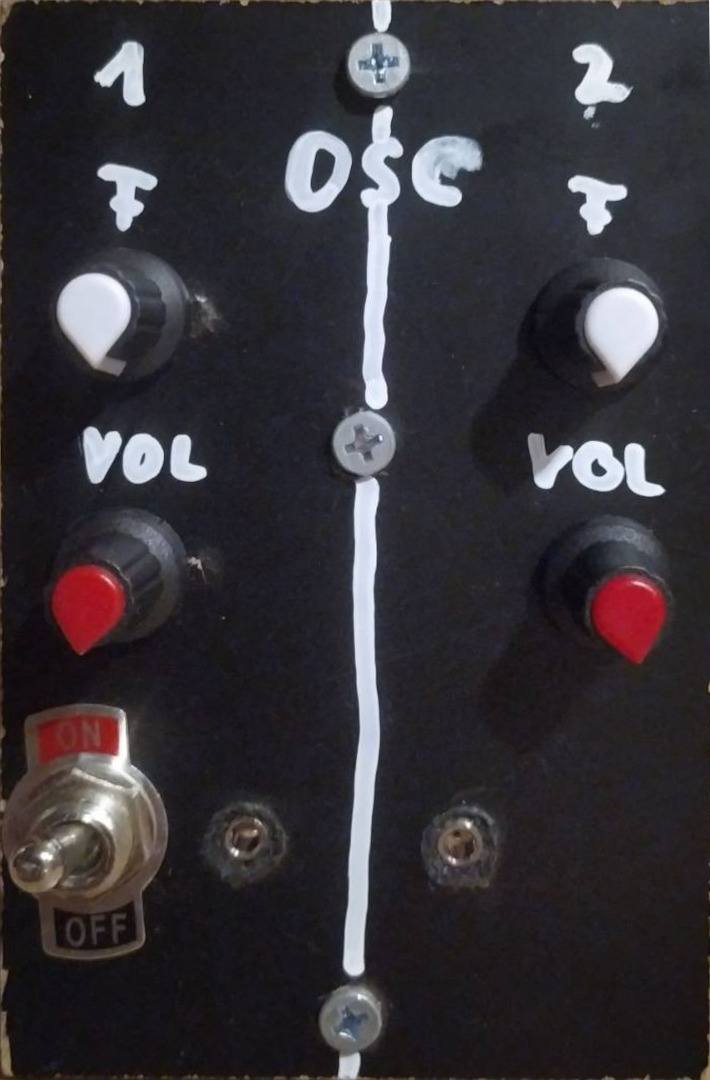
\includegraphics[width=120px]{/home/felixp/Documents/diplomarbeit/dokumentation/figures/modules/oscillator.jpg}
\caption{Deckplatte unseres Oszillator-Moduls}
\end{figure}

\subsection{Spezifikationen}
\label{sec:org0410079}
Oszillator 1:
\begin{itemize}
\item Spannung: bis zu \SI{\pm10}{\volt}
\item Frequenzbereich: \SI{40}{\hertz} bis \(\approx\)\SI{2000}{\hertz}
\end{itemize}

Oszillator 2:
\begin{itemize}
\item Spannung: bis zu \SI{\pm10}{\volt}
\item Frequenzbereich: \SI{25}{\hertz} bis \(\approx\)\SI{2000}{\hertz}
\end{itemize}

\subsection{Elektronik}
\label{sec:orgdf8aba6}
Als Grundlage dient ein einfacher "`Resistor-Capacitor"' Schwingkreis, welcher einen Schmitt-Trigger nutzt. Das resultierende Signal wird durch einen Spannungsfolger gepuffert, da sonst die Oszillation zusammenbricht. Danach wird das Signal AC gekoppelt, um das positive Offset der Oszillation zu entfernen und ein weiteres Mal gepuffert. Darauf folgt ein einfacher variabler Spannungsteiler als Dämpfungsglied, um die Amplitude regulieren zu können.

\subsection{Schematics}
\label{sec:org45830e7}

\begin{circuitikz}[european]
\draw{
(0,0) node[ground, anchor=center, name=G]{}
to[cC, invert, name=C1] ++(0,1)
-- ++(0.5,0)
node[schmitt, anchor=in](S){} (S.out)
-- ++(0,1)
to[pR, l_=R1, name=R1] ++(0,1)
(R1.wiper) -- (R1.wiper -| C1)
-- (C1)

(R1.wiper -| C1)
-- ++(0,1)
-- ++(3,0)
-- ++(0,-2)
-- ++(1,0)

node[op amp, anchor=+](OA1){}
(OA1.out) -- ++(0,1.2)
coordinate (T) -- (T -| OA1.-) -- (OA1.-)

(OA1.out)
to[C, name=C2, l=C2] ++(1,0)
-- ++(0,-0.5)
to[R, name=R2, l=R2] ++(0,-1.5)
node[ground]{}
(C2) -- ++(1,0)

node[op amp, anchor=+](OA2){}
(OA2.out) -- ++(0,1.2)
coordinate (T) -- (T -| OA2.-) -- (OA2.-)

(OA2.out) ++(1,-2.5)
node[ground]{}
to[pR, name=R3, l_=R3] ++(0, 3.5)
-- ++(1,0)
++(0.55,0) node[draw]{OUT}
(R3.wiper) -- (R3.wiper -| OA2.out) -- (OA2.out)
};

\end{circuitikz}

\subsection{Benutzung}
\label{sec:orgeb2b2bd}
Das Panel ist aufgeteilt in einen linken und rechten Oszillator, alle Elemente auf einer Seite gehören zu jeweils einem Oszillator. Die oberen beiden Potentiometer dienen zur Steuerung der Frequenz (siehe Abschnitt \ref{frequenz}), die unteren beiden dienen zur Steuerung der Amplitude (siehe Abschnitt \ref{amplitude}) des Signals. Die Audiobuchsen dienen als Output. Der Schalter links oben aktiviert das Modul, die Oszillatoren sind nicht separat voneinander an- und ausschaltbar.
